\section{阶段性成果与证据分级}
\subsection{两组来源，各自保留验证口径}
本报告纳入两组已提供证据。第一组为仓库归档的 2026-09-09 A 段 fast 研究快照，来源是 \code{docs/research/2026-09-09-results.json}；第二组为用户提供的 Core Lab 截图，位于 \code{report/}。两者的候选命名、样本长度与统计口径不同，\important{不合并候选总数、不拼接收益、不声称同一次运行}。截图体现研究方法的阶段性应用，其原始数据与可执行日志尚未随图提供。

\begin{table}[ht]
\centering\small
\begin{tabularx}{\textwidth}{lXX}
\toprule
证据层级 & 已观察到什么 & 可以支持什么 \\
\midrule
可读取的归档 JSON & 11 个候选、表达式、IC 区间、父子关系、探索判定 & 对固定快照进行重统计与审查 \\
Core Lab 截图 & 条件因子、父子增量、重复切分、晋级/观察/剔除与规律账本 & 展示研究过程与下一轮候选合同 \\
独立确认与交易验证 & 当前两组材料未提供完成证据 & 不能推断正式 alpha 或实盘收益 \\
\bottomrule
\end{tabularx}
\caption{阶段成果的来源与可支持的结论。}
\end{table}

\subsection{AURORA 归档：研究闭环已有可审查产物}
快照记录 13 次尝试、210 次总额度与 11 个完成候选。其中 6 个为 UNDECIDABLE、5 个为 FAIL，独立确认数为 0。按逐候选 lineage 重计，可见 4 个有父结构的子代，其中 3 个 horizontal、1 个 cross\_family。顶层 evolution 汇总计数与这些逐条记录不一致，因此本报告保留原文件，使用逐候选记录计算子代数，并在制图来源清单中记录差异。

这批产物证明系统可以产出冻结表达式、测量结果、拒绝证据和可追溯的父子结构，而不是已经发现可交易 alpha。C010 的高换手条件是预设条件表达，不能统计为本轮自动森林发现；该归档尚无自动条件规则。C011 的训练反向线索与后续段方向不一致，不能仅凭训练负 IC 宣布稳定反向因子。
\begin{figure}[ht]
\centering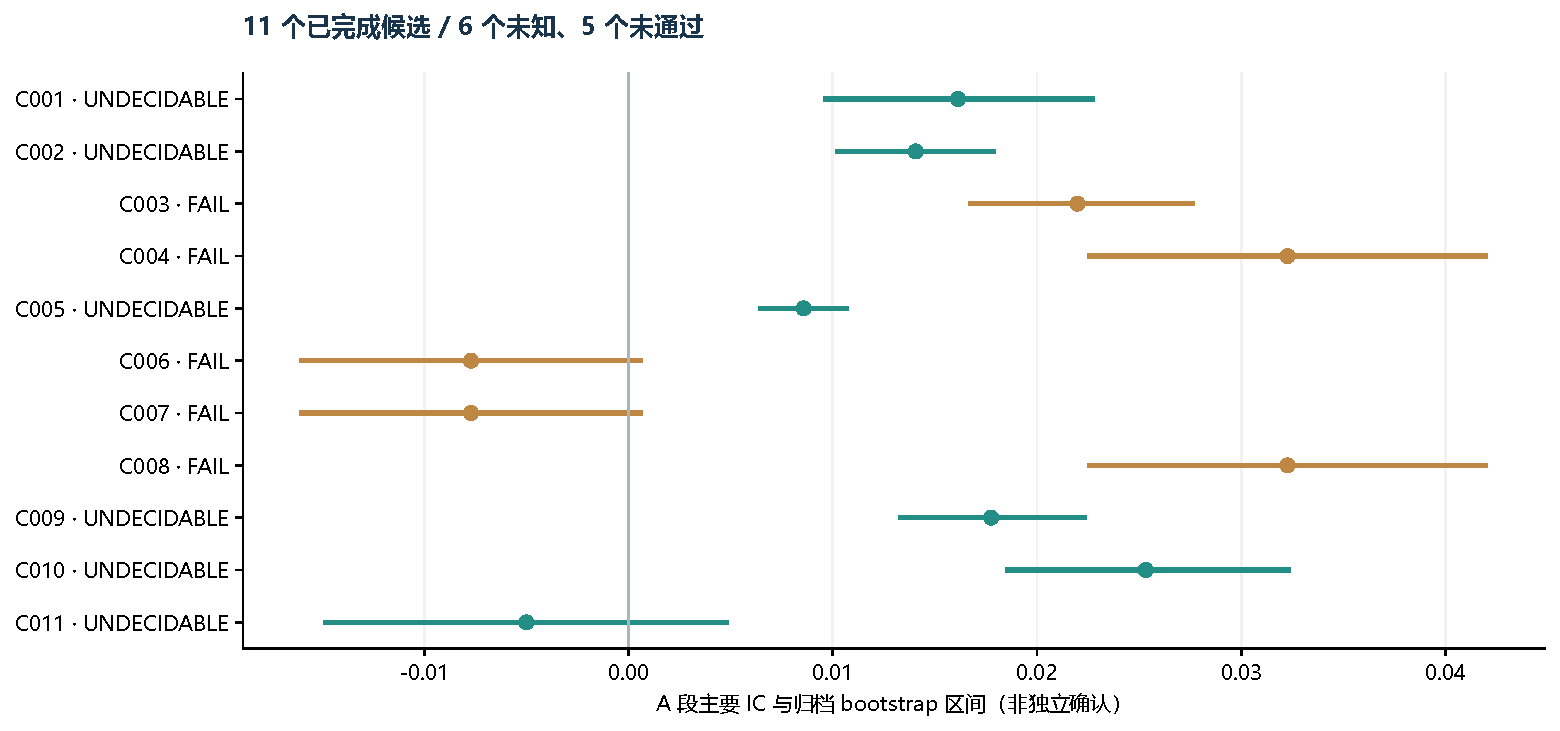
\includegraphics[width=.96\textwidth]{figures/archived_results.pdf}
\caption{归档候选的主要 IC 与原始 bootstrap 区间。绿色为未知，金色为未通过；颜色不代表收益排名。各候选持有期未必相同，图用于证据审查而非严格横向优选。}
\end{figure}

\subsection{Core Lab 案例：条件交互与父子增量}
截图中的候选 \code{CORE170-8EB14F14ED32} 以 \code{pre\_gap\_1d} 为基础，冻结正向、3 日 horizon，并叠加两个区域条件：换手异常相对市场位次不超过 q0.80（图示切点 0.8094），五日收益相对历史位次超过 q0.80（图示切点 0.9）。截图显示第一轮搜索累计两个 gate，说明研究对象从单一信号进入了\important{基础信号与市场状态的交互区域}。

训练区域的父结构 IC 为 0.0210019，条件子结构 IC 为 0.149155，其余区域 IC 为 0.0158302。区域样本数量发生变化，这不是相同样本上净收益提升的证明；其价值在于提出一个明确的下一轮区域假设。训练段仅 25 日、2,201 stock-days，验证段仅 9 日、1,112 stock-days。验证 IC 为 0.0793042、HAC $t$ 为 0.904779，方向虽一致，证据强度仍有限。

\begin{figure}[ht]
\centering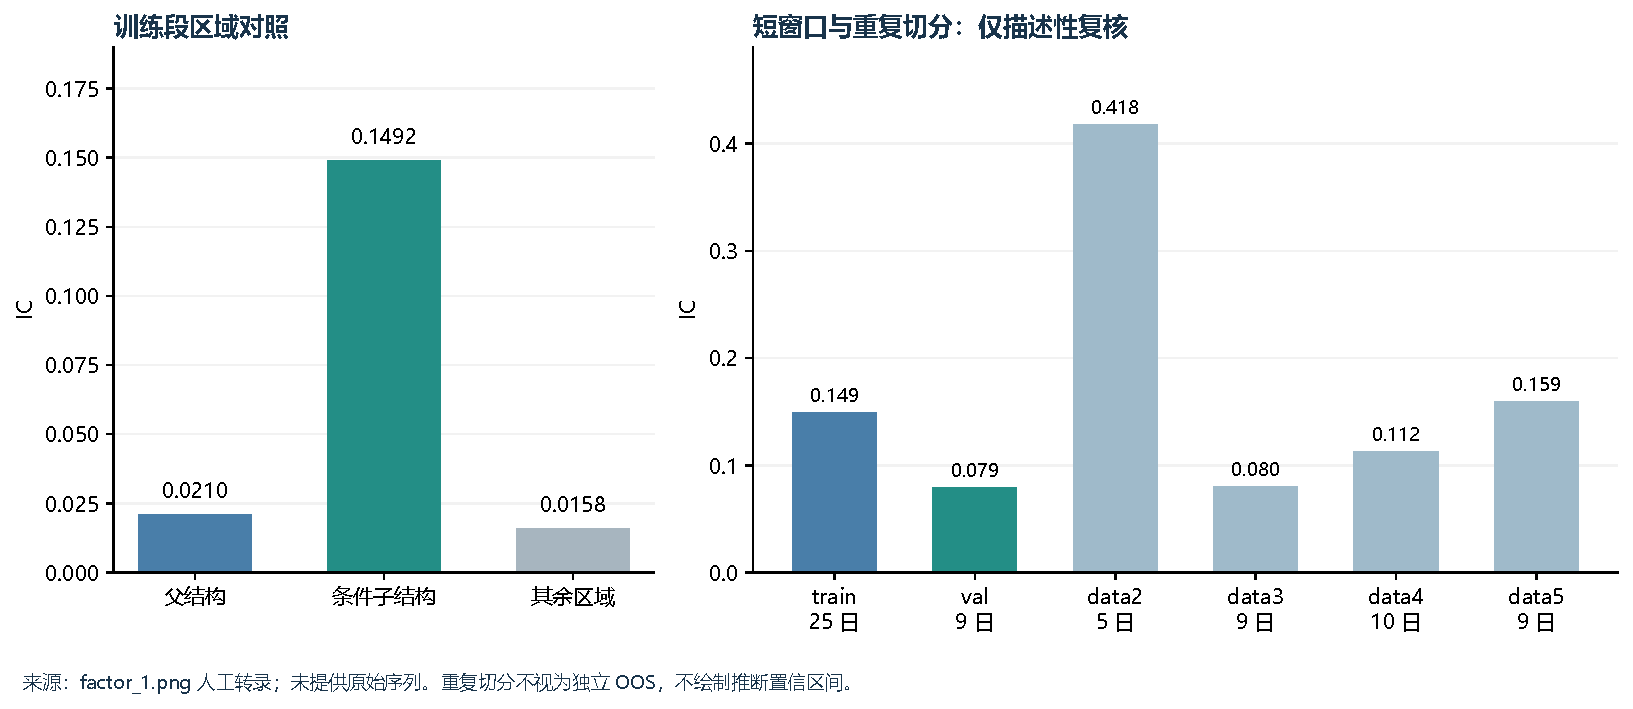
\includegraphics[width=\textwidth]{figures/corelab_case.pdf}
\caption{从用户截图逐值转录的案例。右图 data2--data5 为重复切分标签，不能当作四个独立未见市场。图不补造置信区间，也不把区域 IC 换算为年化收益。}
\end{figure}

\begin{table}[ht]
\centering\small
\begin{tabular}{lrrrr}
\toprule
分段 & IC & HAC $t$ & 交易日 & stock-days \\
\midrule
train & 0.149155 & 2.594850 & 25 & 2201 \\
val & 0.079304 & 0.904779 & 9 & 1112 \\
data2 & 0.417893 & 9.051220 & 5 & 370 \\
data3 & 0.080034 & 0.998685 & 9 & 1341 \\
data4 & 0.112425 & 0.803779 & 10 & 768 \\
data5 & 0.159068 & 1.739080 & 9 & 566 \\
\bottomrule
\end{tabular}
\caption{案例复核值，来源为 factor\_1.png；极短窗口与选择后统计限制其解释范围。}
\end{table}

\subsection{规律账本：把筛选结果反馈为下一轮合同}
\code{factor\_2.png} 的发现后机制解释将该区域描述为消息含义与交易状态/关注结构的交互，并指出它适合作为下一轮 root 合同，而不是事前先验或独立因果结论。\code{law.png} 同时记录 drop 与 observe：例如训练/验证方向翻转、横向强度不足、样本可交易性不足，均有对应理由。

这种记录具有研究价值：失败并非从排行榜消失，而是以边界条件和证据冲突回到下一轮调度。截图里的 promote 表示继续研究的筛选动作，不等于正式 PASS。截图自身也注明 repeated-split 非独立 OOS，以及 CAR、候选内 R-learner 需后续补充；报告沿用这些限制。

\begin{figure}[p]
\centering
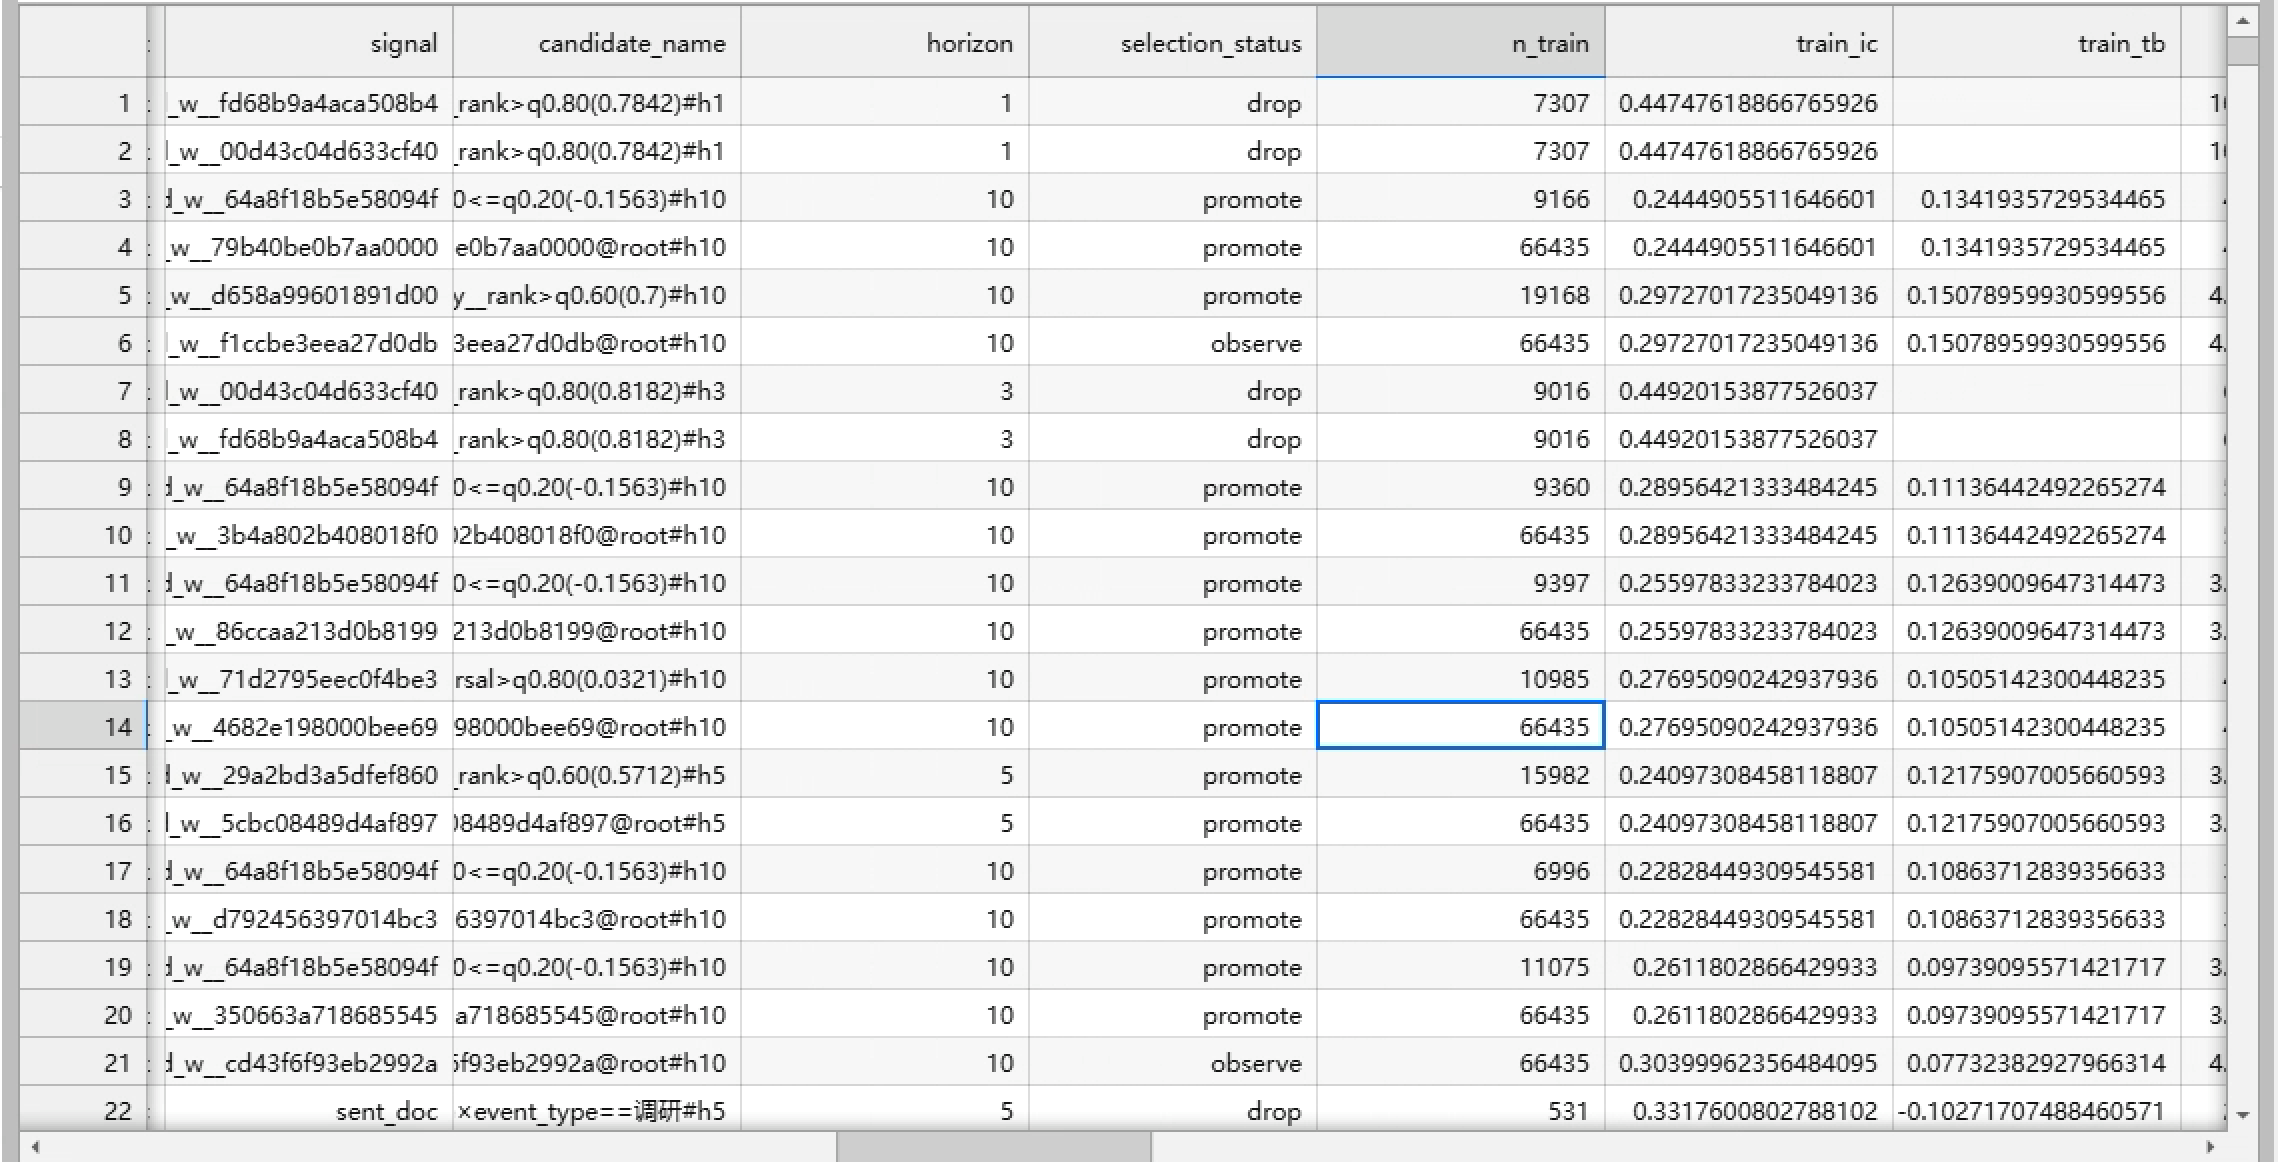
\includegraphics[width=\textwidth,height=.36\textheight,keepaspectratio]{../report/all_factor_show.png}
\caption{原始候选表截屏：同时保留 promote、observe、drop。截图不完整，因此不据此推算候选总量或晋级率。}
\vspace{.8em}
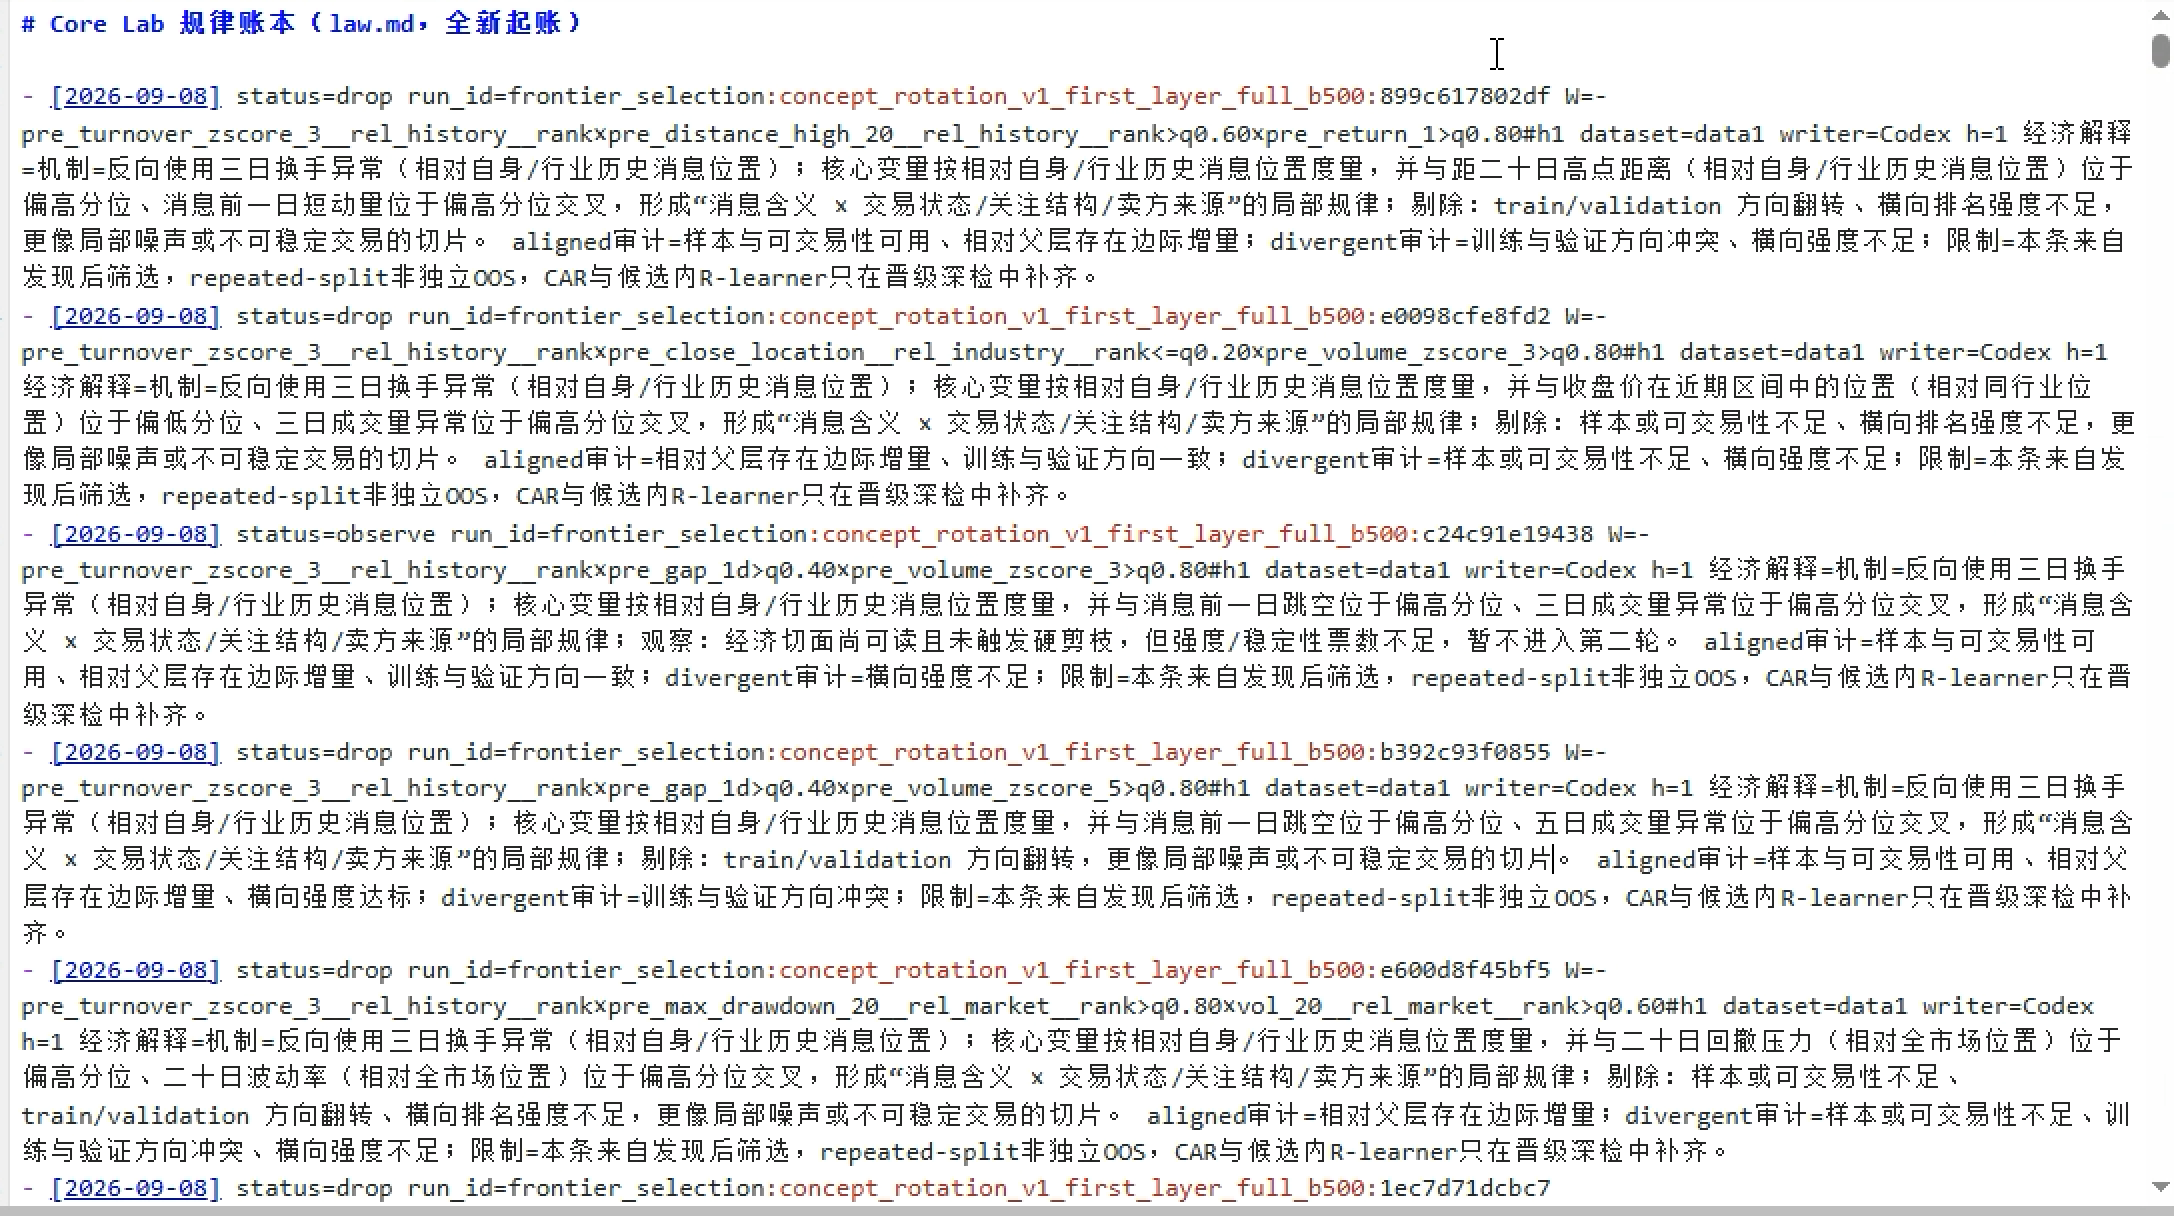
\includegraphics[width=\textwidth,height=.36\textheight,keepaspectratio]{../report/law.png}
\caption{原始规律账本截屏：剔除原因、证据一致与冲突、发现后解释被保留。高清原图随仓库交付。}
\end{figure}
\clearpage